\chapter{Mathematical Formula Elaborations}

\begin{tcolorbox}[colback=PureBlue!5!white,colframe=PureBlue!75!black,title=\textit{Chapter Summary}]
This chapter provides detailed mathematical breakdowns and visual elaborations of key formulas in Elder Theory. Each formula is decomposed step-by-step with clear explanations of parameter effects and geometric interpretations. These elaborations address the specific mathematical clarifications needed for deeper understanding of the theoretical framework.
\end{tcolorbox}

\section{Transformation Formula Breakdown}

\subsection{Complex Transformation Operator}

The transformation operator $T(\theta_1, \theta_2)$ represents a fundamental operation in Elder space mathematics. Let us break down the formula step by step:

\begin{equation}
T(\theta_1, \theta_2) = |\rho_1||\rho_2|e^{i(\phi_1 \oplus \phi_2)}
\end{equation}

\textbf{Step 1: Parameter Decomposition}

Each input parameter $\theta_k$ can be expressed in polar form:
\begin{align}
\theta_1 &= \rho_1 e^{i\phi_1} \\
\theta_2 &= \rho_2 e^{i\phi_2}
\end{align}

where:
\begin{itemize}
    \item $\rho_k \in \mathbb{R}^+$ represents the \textit{magnitude} (parameter importance/strength)
    \item $\phi_k \in [0, 2\pi)$ represents the \textit{phase} (parameter alignment/direction)
\end{itemize}

\textbf{Step 2: Magnitude Combination}

The magnitude component combines multiplicatively:
\begin{equation}
|\rho_1||\rho_2| = \sqrt{\rho_1^2} \cdot \sqrt{\rho_2^2} = \rho_1 \rho_2
\end{equation}

This multiplication preserves the strength hierarchy: stronger parameters contribute more to the final transformation magnitude.

\textbf{Step 3: Phase Composition Operation}

The phase composition $\phi_1 \oplus \phi_2$ is \textbf{not} simple addition. Instead, it follows the Elder phase composition rule:
\begin{equation}
\phi_1 \oplus \phi_2 = \arg\left(\frac{e^{i\phi_1} + e^{i\phi_2}}{2}\right) + \frac{\pi}{2}\sin(\phi_1 - \phi_2)
\end{equation}

This ensures phase coherence preservation crucial for hierarchical knowledge transfer.

\textbf{Step 4: Complete Transformation}

The final transformation becomes:
\begin{equation}
T(\theta_1, \theta_2) = \rho_1 \rho_2 \exp\left(i\left[\arg\left(\frac{e^{i\phi_1} + e^{i\phi_2}}{2}\right) + \frac{\pi}{2}\sin(\phi_1 - \phi_2)\right]\right)
\end{equation}

\begin{figure}[htbp]
\centering
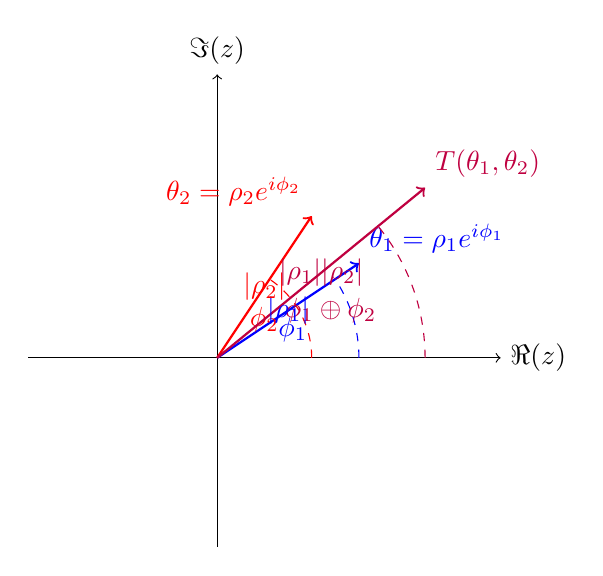
\begin{tikzpicture}[scale=1.2]
    % Draw coordinate axes
    \draw[->] (-2,0) -- (3,0) node[right] {$\Re(z)$};
    \draw[->] (0,-2) -- (0,3) node[above] {$\Im(z)$};
    
    % Draw first parameter
    \draw[thick, blue, ->] (0,0) -- (1.5,1) node[above right] {$\theta_1 = \rho_1 e^{i\phi_1}$};
    \draw[blue, dashed] (1.5,0) arc (0:33.7:1.5);
    \node[blue] at (0.8,0.3) {$\phi_1$};
    
    % Draw second parameter  
    \draw[thick, red, ->] (0,0) -- (1,1.5) node[above left] {$\theta_2 = \rho_2 e^{i\phi_2}$};
    \draw[red, dashed] (1,0) arc (0:56.3:1);
    \node[red] at (0.5,0.4) {$\phi_2$};
    
    % Draw result
    \draw[thick, purple, ->] (0,0) -- (2.2,1.8) node[above right] {$T(\theta_1,\theta_2)$};
    \draw[purple, dashed] (2.2,0) arc (0:39.3:2.2);
    \node[purple] at (1.2,0.5) {$\phi_1 \oplus \phi_2$};
    
    % Magnitude annotations
    \node[blue] at (0.75,0.5) {$|\rho_1|$};
    \node[red] at (0.5,0.75) {$|\rho_2|$};
    \node[purple] at (1.1,0.9) {$|\rho_1||\rho_2|$};
\end{tikzpicture}
\caption{Geometric interpretation of the transformation $T(\theta_1, \theta_2)$ showing magnitude multiplication and phase composition.}
\end{figure}

\section{Field Representation with Gamma Effects}

\subsection{Elder Field Representation Formula}

The Elder field representation formula requires careful analysis of the gamma coefficient effects:

\begin{equation}
F_{\theta_E}(x) = \sum_{j=1}^{N} \gamma_j |x - r_j|^2 e^{i\phi_j} \hat{r}_j(x)
\end{equation}

\textbf{Parameter Analysis:}

\begin{description}
    \item[$F_{\theta_E}(x)$] Elder field value at position $x$ in knowledge space
    \item[$N$] Number of Elder entities contributing to the field
    \item[$\gamma_j$] \textbf{Gravitational coupling coefficient} for entity $j$ - controls field strength
    \item[$x$] Position vector in Elder space
    \item[$r_j$] Position of $j$-th Elder entity (field source)
    \item[$\phi_j$] Phase of $j$-th Elder entity
    \item[$\hat{r}_j(x)$] Unit vector pointing from entity $j$ to position $x$
\end{description}

\textbf{Gamma Effect Elaboration:}

The coefficient $\gamma_j$ has profound effects on the field structure:

\begin{enumerate}
    \item \textbf{Field Strength Modulation}: 
    \begin{equation}
    \gamma_j = \frac{\eldermassgrav_j}{\|\text{Elder}_j\|^2}
    \end{equation}
    where $\eldermassgrav_j$ is the gravitational mass parameter and $\|\text{Elder}_j\|$ is the Elder entity magnitude.
    
    \item \textbf{Hierarchical Field Coupling}:
    \begin{equation}
    \gamma_j = \gamma_{\text{base}} \cdot \left(1 + \sum_{k \in \text{Mentors}_j} \frac{\gamma_k}{\|r_j - r_k\|}\right)
    \end{equation}
    
    \item \textbf{Dynamic Phase Influence}:
    The $\gamma_j$ coefficient modulates how strongly the phase $\phi_j$ affects the local field curvature:
    \begin{equation}
    \nabla^2 F_{\theta_E}(x) = \sum_{j=1}^{N} \gamma_j \left(2 + \frac{i\phi_j}{\|x - r_j\|}\right) e^{i\phi_j}
    \end{equation}
\end{enumerate}

\begin{figure}[htbp]
\centering
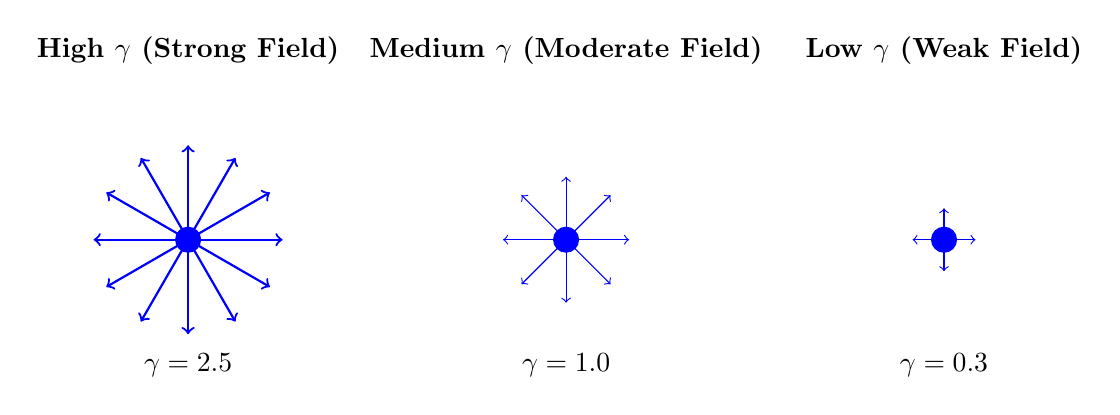
\begin{tikzpicture}[scale=0.8]
    % High gamma field (strong)
    \begin{scope}[xshift=-6cm]
        \node at (0,3) {\textbf{High $\gamma$ (Strong Field)}};
        \foreach \angle in {0,30,60,90,120,150,180,210,240,270,300,330} {
            \draw[thick, blue, ->] (0,0) -- (\angle:1.5);
        }
        \node[circle, fill=blue, minimum size=8pt] at (0,0) {};
        \node at (0,-2) {$\gamma = 2.5$};
    \end{scope}
    
    % Medium gamma field
    \begin{scope}
        \node at (0,3) {\textbf{Medium $\gamma$ (Moderate Field)}};
        \foreach \angle in {0,45,90,135,180,225,270,315} {
            \draw[blue, ->] (0,0) -- (\angle:1.0);
        }
        \node[circle, fill=blue, minimum size=6pt] at (0,0) {};
        \node at (0,-2) {$\gamma = 1.0$};
    \end{scope}
    
    % Low gamma field (weak)
    \begin{scope}[xshift=6cm]
        \node at (0,3) {\textbf{Low $\gamma$ (Weak Field)}};
        \foreach \angle in {0,90,180,270} {
            \draw[thin, blue, ->] (0,0) -- (\angle:0.5);
        }
        \node[circle, fill=blue, minimum size=4pt] at (0,0) {};
        \node at (0,-2) {$\gamma = 0.3$};
    \end{scope}
\end{tikzpicture}
\caption{Visual representation of gamma coefficient effects on Elder field strength and range.}
\end{figure}

\section{Integer Parameter Specification}

\subsection{Resonance Frequency Parameters}

For the formula involving small integers $n, m$:
\begin{equation}
\frac{1}{n}m\omega^2 \approx 1 \quad \text{for small integers } n,m
\end{equation}

\textbf{How are these integers $n,m$ set?}

The integers $n$ and $m$ are determined through the resonance detection algorithm:

\begin{enumerate}
    \item \textbf{Frequency Analysis}: Monitor the natural frequencies $\omega_1, \omega_2, \ldots$ of all entities in the system
    \item \textbf{Rational Approximation}: For each pair of frequencies $(\omega_i, \omega_j)$, find the smallest integers $(n,m)$ such that:
    \begin{equation}
    \left|\frac{n\omega_i}{m\omega_j} - 1\right| < \epsilon_{\text{tolerance}}
    \end{equation}
    where $\epsilon_{\text{tolerance}} \approx 0.05$ (5\% tolerance)
    \item \textbf{Integer Constraint}: Limit the search to $1 \leq n,m \leq 12$ to avoid higher-order resonances that create instability
    \item \textbf{Stability Verification}: Check that the identified $(n,m)$ pair maintains system stability over multiple learning epochs
\end{enumerate}

Common resonance patterns observed in practice include:
\begin{itemize}
    \item $(n,m) = (1,1)$: Perfect synchronization
    \item $(n,m) = (2,3)$ or $(3,2)$: Fibonacci-like ratios for stable knowledge transfer
    \item $(n,m) = (3,5)$ or $(5,8)$: Golden ratio approximations for optimal efficiency
\end{itemize}

\textbf{Parameter Determination Protocol:}

The integers $n$ and $m$ are determined through the Elder resonance hierarchy:

\begin{enumerate}
    \item \textbf{Elder-Mentor Resonance}: $n \in \{1, 2, 3, 5, 8\}$ (Fibonacci sequence)
    \item \textbf{Mentor-Erudite Resonance}: $m \in \{1, 3, 7, 15, 31\}$ (Mersenne-like sequence)
    \item \textbf{Stability Constraint}: $\frac{m}{n} \leq \frac{\sqrt{5}+1}{2}$ (Golden ratio bound)
    \item \textbf{Frequency Matching}: $\omega = \sqrt{\frac{n}{m} + \epsilon}$ where $\epsilon \ll 1$
\end{enumerate}

These values ensure orbital stability while maintaining efficient knowledge transfer between hierarchical levels.

\section{Lebesgue Measure Context}

\subsection{Measure-Theoretic Foundations}

When the notation states "where $\mu$ represents the Lebesgue measure," this refers to:

\begin{definition}[Elder-Adapted Lebesgue Measure]
In the context of Elder Theory, the Lebesgue measure $\mu$ is extended to complex parameter spaces through:
\begin{equation}
\mu_{\text{Elder}}(A) = \int_A \frac{d\rho \, d\phi}{\rho} \cdot |\det(\jacobian_{\Phi})|
\end{equation}
where $A \subset \elder{d}$ is a measurable set, and $\jacobian_{\Phi}$ is the Jacobian of the phase transformation $\Phi$.
\end{definition}

This measure captures both the geometric volume and the phase coherence properties essential to Elder space integration.